\documentclass{report}

\usepackage[utf8]{inputenc}
\usepackage[english, russian]{babel}
\usepackage{geometry}
\usepackage{listings}
\usepackage[T2A]{fontenc}
\usepackage[14pt]{extsizes}
\usepackage{color}
\usepackage{graphicx}
\usepackage[titles]{tocloft}
\usepackage[hyphens]{url}


\geometry{a4paper,top=2cm,bottom=2cm,left=2cm,right=1.5cm}
\setlength{\parskip}{0.5cm}
\setcounter{tocdepth}{4}
\setcounter{secnumdepth}{4}
\sloppy

\definecolor{darkgreen}{rgb}{0.0, 0.5, 0.0}
\lstset{
    language=C++,
    basicstyle=\footnotesize,
    numbers=left,
    numberstyle=\tiny,
    numberfirstline=true,
    numbersep=5pt,
    keywordstyle=\color{blue}\bfseries,
    commentstyle=\color{darkgreen},
    stringstyle=\color{red},
    showspaces=false,
    showstringspaces=false,
    captionpos=t,
    breaklines=true,
    breakatwhitespace=false,
    extendedchars=true,
    frame=tb,
    title=\lstname,
}

\begin{document}
    \begin{titlepage}

        \begin{center}
            \textbf{Федеральное государственное автономное образовательное учреждение высшего образования} \\
            "Национальный исследовательский Нижегородский государственный университет им. Н.И. Лобачевского" (ННГУ) \\
            \textbf{Институт информационных технологий, математики и механики}

            \vspace{\fill}

            \textbf{\LargeОтчет по лабораторной работе \\}
            \textbf{\large\\ «Линейная фильтрация изображений (горизонтальное разбиение). Ядро Гаусса 3x3»}

            \vspace{\fill}

            \hfill\parbox{8cm}{
                \hspace*{5cm}\hspace*{-5cm}\textbf{Выполнил:} \\ Студент группы 381708-1 \\ Оболенский Арсений Андреевич \\ \\ \\
                \hspace*{5cm}\hspace*{-5cm}\textbf{Проверил:}\\ Доцент кафедры МОСТ, \\ кандидат технических наук \\ Сысоев А. В.
                \hbadness=20000
            }

            \vspace{\fill}

            Нижний Новгород \\ 2020 г.
        \end{center}

    \end{titlepage}

    % =============================================
    % Оглавление
    % =============================================
    \setcounter{page}{2}
    \setlength{\cftsecindent}{0em}
    \setlength{\cftsubsecindent}{1.25em}
    \setlength{\cftsubsubsecindent}{2.5em}
    \setlength{\cftsubsubsecnumwidth}{1.25em}
    \tableofcontents


    \newpage
    % =============================================
    % Введение
    % =============================================
    \section*{Введение}
    \addcontentsline{toc}{section}{Введение}
    \par Фильтр Гаусса - это метод фильтрации изображений, который использует нормальное распределение (также называемое Гауссовым распределением) для вычисления преобразования, применяемого к каждому пикселю изображения. Данный фильтр используется для создания эффекта размытия изображения, а также для того, чтобы уменьшить шумы на изображении.
    \par Тот факт, что данный фильтр применяется к каждому пикселю в отдельности независимо от остальных, открывает возможности для существенного ускорения его работы путем распараллеливания вычислений между разными ядрами процессора.
    \par Целью данной работы является изучение алгоритма линейной фильтрации с помощью фильтра Гаусса и реализация последовательной и нескольких параллельных версий алгоритма с использованием разных технологий выполнения параллельных вычислений.


    \newpage
    % =============================================
    % 1. Постановка задачи
    % =============================================
    \section*{1. Постановка задачи}
    \addcontentsline{toc}{section}{1. Постановка задачи}

    \par В ходе данной лабораторной работы требуется:
    \begin{itemize}
        \item изучить фильтрацию методом Гаусса;
        \item написать последовательную реализацию алгоритма, выполняющего фильтрацию;
        \item написать параллельные реализации алгоритма, выполняющего фильтрацию, с помощью OpenMP, TBB и потоков из стандартной библиотеки языка C++ (\verb|std::thread|);
        \item выполнить сравнение и сделать выводы об эффективности написанных реализаций;
        \item проверить корректность работы алгоритма.
    \end{itemize}


    \newpage
    % =============================================
    % 2. Описание алгоритма
    % =============================================
    \section*{2. Описание алгоритма}
    \addcontentsline{toc}{section}{2. Описание алгоритма}

    \par Фильтр Гаусса - это широко используемый в обработке изображений фильтр. Главным образом он используется для устранения шумов на изображении и сделать эффект размытия. Гауссово размывание применяет функцию Гаусса (\ref{eq:normal_dist}), которая также выражает нормальное распределение в математической статистике, к каждому пикселю в изображении.
    \begin{equation}
        \label{eq:normal_dist}
        \frac{1}{\sigma\sqrt{2\pi}}\exp\left(-\frac{x^2 + y^2}{2\sigma^2}\right)
    \end{equation}
    \par Генерируется ядро размером 3x3 с использованием вышеприведенной формулы таким образом, чтобы сумма всех чисел в ядре была равна единице для того, чтобы не делать изображение ярче или темнее. Далее требуется применить ядро к каждому пикселю изображения.
    \begin{figure}[htbp]
        \centering
        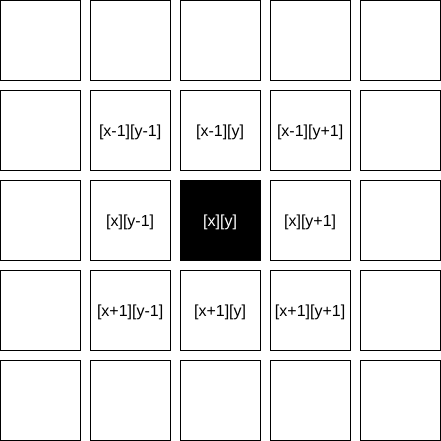
\includegraphics[width=0.55\textwidth]{../../../../modules/reports/obolenskiy_a_gaussian_image_filtering/grid.png}
        \caption{Расчет цвета одного пикселя изображения}
    \end{figure}
    \par Новый цвет для пикселя с индексами [x][y] будет равен сумме произведений значения цветовой компоненты каждого из пикселей на соответствующее значение из ядра ($pixel[x][y] * kernel[x][y]$). Полученное значение нормализуется так, чтобы оно оказалось в диапазоне [0, 255].


    \newpage
    % =============================================
    % 3. Описание схемы распараллеливания
    % =============================================
    \section*{3. Описание схемы распараллеливания}
    \addcontentsline{toc}{section}{3. Описание схемы распараллеливания}

    \par Для эффективного распределения задач по потокам использовалась схема горизонтального разбиения. Она выглядит следующим образом: изображение разбивается на N горизонтальных полосок, где N - число потоков, на которые мы хотим распределить вычисления, с приблизительно равной высотой. Далее в каждом потоке отдельно обрабатывается каждая из N частей изображения.
    \begin{figure}[htbp]
        \centering
        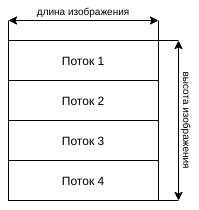
\includegraphics[width=0.45\textwidth]{../../../../modules/reports/obolenskiy_a_gaussian_image_filtering/thread_schema.png}
        \caption{Схема распараллеливания для четырех потоков}
    \end{figure}


    \newpage
    % =============================================
    % 4. Описание программной реализации
    % =============================================
    \section*{4. Описание программной реализации}
    \par Данный раздел содержит краткие описания схем параллельного выполнения. Полный код можно найти в приложении.
    \addcontentsline{toc}{section}{4. Описание программной реализации}
    \subsection*{4.1. Описание реализации с использованием OpenMP}
    \par Для распараллеливания алгоритма при помощи технологии OpenMP использовалась директива препроцессора \verb|#pragma omp parallel for|. \\
    Она позволяет разделить выполнение цикла, который итерируется по строкам изображения, на N примерно равных частей, как и описано в схеме распараллеливания.
    \addcontentsline{toc}{subsection}{4.1. Описание реализации с использованием OpenMP}
    \subsection*{4.2. Описание реализации с использованием TBB}
    \addcontentsline{toc}{subsection}{4.2. Описание реализации с использованием TBB}
    \par Чтобы выполнить данный алгоритм параллельно с помощью TBB, использовалась функция \verb|tbb::parallel_for|. Она позволяет выполнить автоматическое разделение изображения на порции вычислений при помощи планировщика библиотеки TBB. \\
    Чтобы добиться разбиения изображения именно по строкам, нужно передать в функцию \verb|tbb::parallel_for| объект \verb|tbb::blocked_range<int>(0, rows)|, где rows - это количество строк в изображении. Также в \verb|tbb::parallel_for| передается функтор, который выполняет, собственно, саму операцию фильтрации для каждого пикселя из области, определенной итерационным пространством \verb|tbb::blocked_range|.
    \subsection*{4.3. Описание реализации с использованием std::thread}
    \addcontentsline{toc}{subsection}{4.3. Описание реализации с использованием std::thread}
    \par Для выполнения параллельной фильтрации изображения с использованием \verb|std::thread| из стандартной библиотеки языка C++, нужно разделить изображение на примерно равные части самостоятельно. \\
    В цикле с количеством итераций, равным количеству потоков, будем создавать объекты класса \verb|std::thread| и передавать им лямбда-функцию, которая выполняет полезную работу по фильтрации для каждого пикселя из области, и саму область (два целых числа, которые описывают строку, с которой начать фильтрацию в данном потоке, и строку, на которой нужно закончить фильтрацию).
    После этого нужно дождаться окончания выполнения всех потоков, поэтому в главном потоке нужно на каждом объекте \verb|std::thread| вызывается метод \verb|join()|.


    \newpage
    % =============================================
    % 5. Результаты экспериментов и описание подтверждения корректности
    % =============================================
    \section*{5. Результаты экспериментов и описание подтверждения корректности}
    \addcontentsline{toc}{section}{5. Результаты экспериментов и описание подтверждения корректности}
    \par Конфигурация системы:
    \begin{itemize}
        \item Процессор: AMD FX-8370E @ 3.7GHz (8 ядер / 8 потоков)
        \item Оперативная память: 16 GB (DDR3, 1600MHz)
        \item Операционная система: Ubuntu 20.04
        \item Компилятор: g++ 9.3.0
    \end{itemize}
    \par Сбор экспериментальных данных производился на случайном изображении размером 3840x2160.
    \begin{table}[htbp]
        \centering
        \begin{tabular}{|c|c|c|c|c|c|c|}
            \hline
                             & 1       & 2       & 3       & 4        & 6        & 8        \\ \hline
            Последовательная & \multicolumn{6}{c|}{3.00508}                                 \\ \hline
            OpenMP           & 2.98192 & 1.54635 & 1.00003 & 0.757113 & 0.598993 & 0.470119 \\ \hline
            TBB              & 2.97817 & 1.51188 & 1.0098  & 0.763663 & 0.576086 & 0.47195  \\ \hline
            std::thread      & 3.10689 & 1.78757 & 1.18321 & 0.903351 & 0.623189 & 0.475944 \\ \hline
        \end{tabular}
        \caption{Результаты экспериментов.}
        \label{tab:results}
        По вертикали - число потоков. \\
        По горизонтали - тестируемая реализация. \\
        Время указано в секундах.
    \end{table}
    \par Для подтверждения корректности используются Unit-тесты с помощью Google Test Framework. Тесты используются как в последовательной, так и в параллельной версии.
    \par Также для проверки корректности используется визуальный анализ полученных после работы алгоритма изображений. А именно:
    \begin{itemize}
        \item При помощи библиотеки OpenCV считывается изображение с диска;
        \item конвертируется в массив пикселей \verb|RGB|;
        \item выполняется фильтрация этого изображения;
        \item и снова с помощью средств OpenCV полученное изображение отображается в отдельном окне (или сохраняется в отдельный файл).
    \end{itemize}
    \par Пример работы визуальной проверки:
    \begin{figure}[htbp]
        \centering
        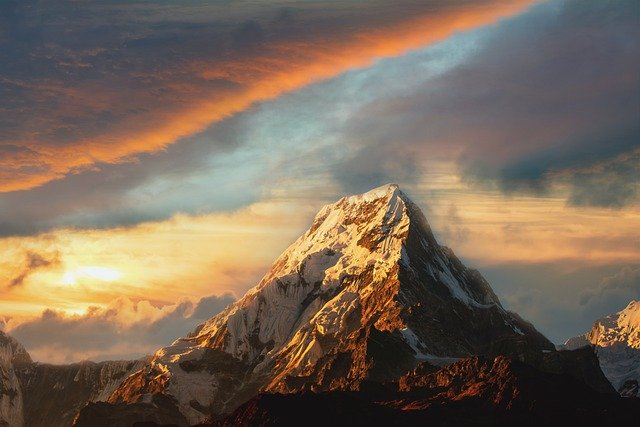
\includegraphics[width=0.99\textwidth]{../../../../modules/reports/obolenskiy_a_gaussian_image_filtering/source.png}
        \caption{Исходное изображение}
    \end{figure}
    \begin{figure}[htbp]
        \centering
        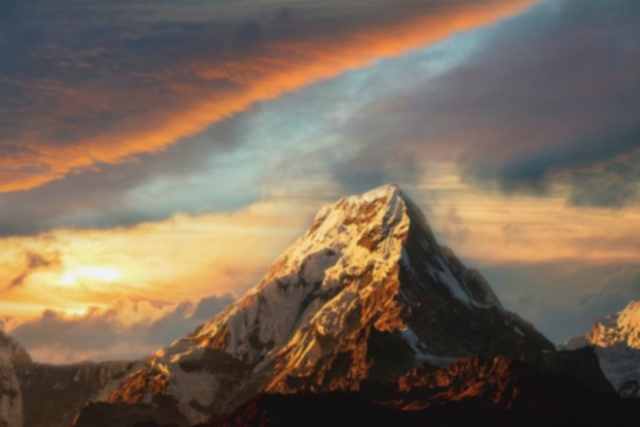
\includegraphics[width=0.99\textwidth]{../../../../modules/reports/obolenskiy_a_gaussian_image_filtering/result.png}
        \caption{Изображение, обработанное фильтром Гаусса с ядром 3х3}
    \end{figure}

    \newpage
    % =============================================
    % Заключение
    % =============================================
    \section*{Заключение}
    \addcontentsline{toc}{section}{Заключение}

    \par В процессе выполнения данных лабораторных работ была изучена фильтрация методом Гаусса, написана последовательная и три параллельные реализации данного алгоритма. Также была проведена визуальная оценка качества работы, оценка скорости работы данных реализаций и написаны тесты для них.
    \par В результате самыми эффективными реализациями оказались те, которые написаны с помощью технологий OpenMP и TBB.

    \newpage
    % =============================================
    % Список литературы
    % =============================================
    \section*{Список литературы}
    \addcontentsline{toc}{section}{Список литературы}
    \begin{enumerate}
        \item Сысоев А.В., Мееров И.Б., Сиднев А.А. Средства разработки параллельных программ для систем с общей памятью. Библиотека Intel Threading Building Blocks. Учебно-методические материалы по программе повышения квалификации «Технологии высокопроизводительных вычислений для обеспечения учебного процесса и научных исследований». Нижний Новгород, 2007, 86 с.
        \item Guide into OpenMP: Easy multithreading programming for C++. URL: \url{https://bisqwit.iki.fi/story/howto/openmp/}
        \item Intel Threading Building Blocks User Guide. URL: \url{https://www.threadingbuildingblocks.org/docs/help/tbb_userguide/parallel_for.html}
        \item Open Computer Vision library documentation. URL: \url{https://docs.opencv.org/4.3.0/index.html}
        \item Турлапов В.Е., Гетманская А.А., Васильев Е.П., Дубровская М.В. Методические указания для проведения лабораторных работ по курсу "КОМПЬЮТЕРНАЯ ГРАФИКА": Учебное пособие. – Нижний Новгород, Национальный Исследовательский Нижегородский государственный университет им. Н.И. Лобачевского, 2018 – 96 с.
    \end{enumerate}

    \newpage
    % =============================================
    % Приложение
    % =============================================
    \section*{Приложение}
    \addcontentsline{toc}{section}{Приложение}

    \subsection*{Исходный код}
    \addcontentsline{toc}{subsection}{Исходный код}

    \subsubsection*{Лабораторная работа №1. Последовательная версия}
    \addcontentsline{toc}{subsubsection}{Лабораторная работа №1. Последовательная версия}
    \lstinputlisting[language=C++, caption=Последовательная версия. Заголовочный файл]{../../../../modules/task_1/obolenskiy_a_gaussian_image_filtering/gaussian_image_filtering.h}
    \lstinputlisting[language=C++, caption=Последовательная версия. Файл с реализацией]{../../../../modules/task_1/obolenskiy_a_gaussian_image_filtering/gaussian_image_filtering.cpp}
    \lstinputlisting[language=C++, caption=Последовательная версия. Файл с тестами]{../../../../modules/task_1/obolenskiy_a_gaussian_image_filtering/main.cpp}

    \newpage
    \subsubsection*{Лабораторная работа №2. Параллельная версия с использованием OpenMP}
    \addcontentsline{toc}{subsubsection}{Лабораторная работа №2. Параллельная версия с использованием OpenMP}
    \lstinputlisting[language=C++, caption=Последовательная версия. Заголовочный файл]{../../../../modules/task_2/obolenskiy_a_gaussian_image_filtering/gaussian_image_filtering.h}
    \lstinputlisting[language=C++, caption=Последовательная версия. Файл с реализацией]{../../../../modules/task_2/obolenskiy_a_gaussian_image_filtering/gaussian_image_filtering.cpp}
    \lstinputlisting[language=C++, caption=Последовательная версия. Файл с тестами]{../../../../modules/task_2/obolenskiy_a_gaussian_image_filtering/main.cpp}

    \newpage
    \subsubsection*{Лабораторная работа №3. Параллельная версия с использованием TBB}
    \addcontentsline{toc}{subsubsection}{Лабораторная работа №3. Параллельная версия с использованием TBB}
    \lstinputlisting[language=C++, caption=Последовательная версия. Заголовочный файл]{../../../../modules/task_3/obolenskiy_a_gaussian_image_filtering/gaussian_image_filtering.h}
    \lstinputlisting[language=C++, caption=Последовательная версия. Файл с реализацией]{../../../../modules/task_3/obolenskiy_a_gaussian_image_filtering/gaussian_image_filtering.cpp}
    \lstinputlisting[language=C++, caption=Последовательная версия. Файл с тестами]{../../../../modules/task_3/obolenskiy_a_gaussian_image_filtering/main.cpp}

    \newpage
    \subsubsection*{Лабораторная работа №4. Параллельная версия с использованием std::thread}
    \addcontentsline{toc}{subsubsection}{Лабораторная работа №4. Параллельная версия с использованием std::thread}
    \lstinputlisting[language=C++, caption=Последовательная версия. Заголовочный файл]{../../../../modules/task_4/obolenskiy_a_gaussian_image_filtering/gaussian_image_filtering.h}
    \lstinputlisting[language=C++, caption=Последовательная версия. Файл с реализацией]{../../../../modules/task_4/obolenskiy_a_gaussian_image_filtering/gaussian_image_filtering.cpp}
    \lstinputlisting[language=C++, caption=Последовательная версия. Файл с тестами]{../../../../modules/task_4/obolenskiy_a_gaussian_image_filtering/main.cpp}

\end{document}
